%___________________________ Q 4.2 ______________________________
\subsection{Show and describe the block diagram used to control the system. (1.5 pts)}
\vspace{10pt}

%%Write your answer here

All simulink models devloped in this part of the course can be seen in this chapter. The model in Figure \ref{fig:plant_interface} represents the plant interface, facilitating the interaction between the physical system and the control model, specifically, sensor data and actuator signals are processed through this interface. The model present in figure \ref{fig:state_estimator} depicts the state estimator, which is responsible for estimating the system states based on sensor inputs and control signals, utilizing a Kalman filter. Lastly, the state feedback controller, shown in Figure \ref{fig:controller_without_integrator}, is tasked with generating the control signals sent to the actuators. This controller does not incorporate integral action, this means that if the motor or gearbox has any type of non moduled dead zones the system will have a steady state error.

To fix this possible problem a new optimal controller with integral action was designed, as we can see in figure \ref{fig:controler_with_integrator}, this new control simply integrates the error of the system as sum to the control signal.

\begin{figure}[H]
    \centering
    \begin{subfigure}{0.47\textwidth}
        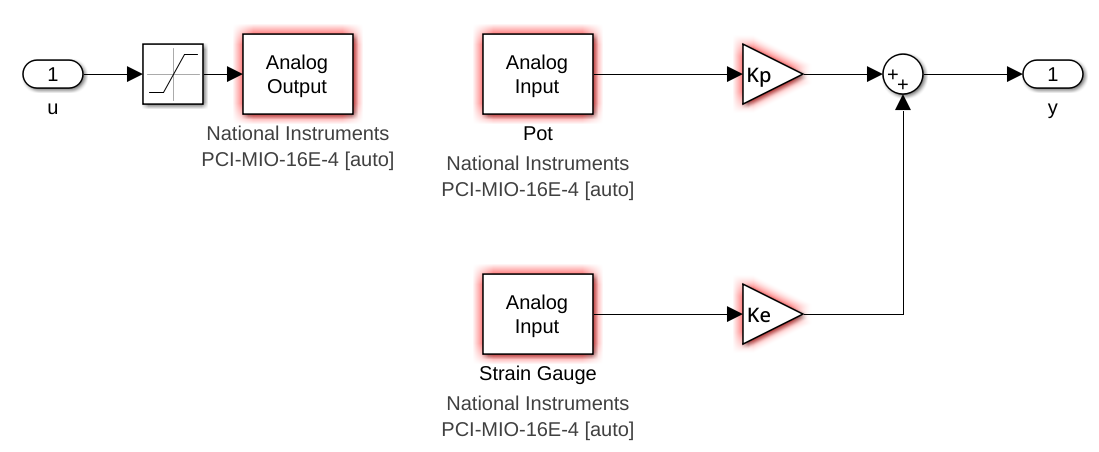
\includegraphics[width=\textwidth]{Figs/Simulink Models/Plant Interface.png}
        \caption{Plant interface}
        \label{fig:plant_interface}
    \end{subfigure}
    \hfill
    \begin{subfigure}{0.37\textwidth}
        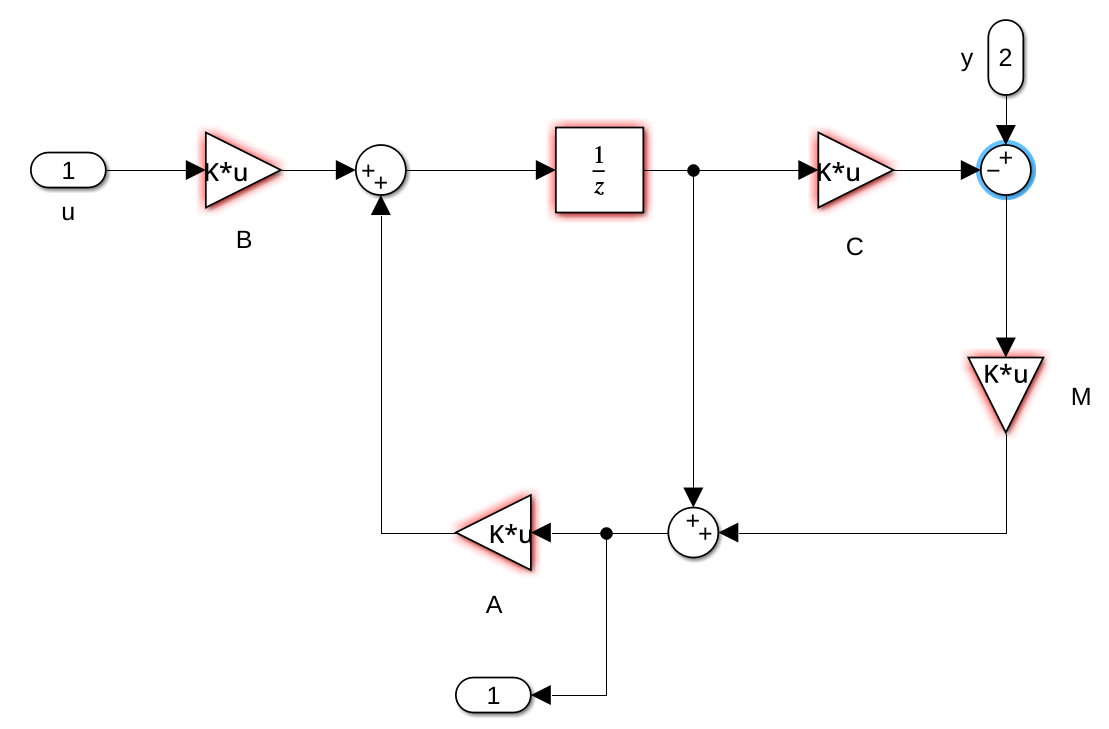
\includegraphics[width=\textwidth]{Figs/Simulink Models/State_Estimator.png}
        \caption{State Estimator}
        \label{fig:state_estimator}
    \end{subfigure}
    \begin{subfigure}{0.95\textwidth}
        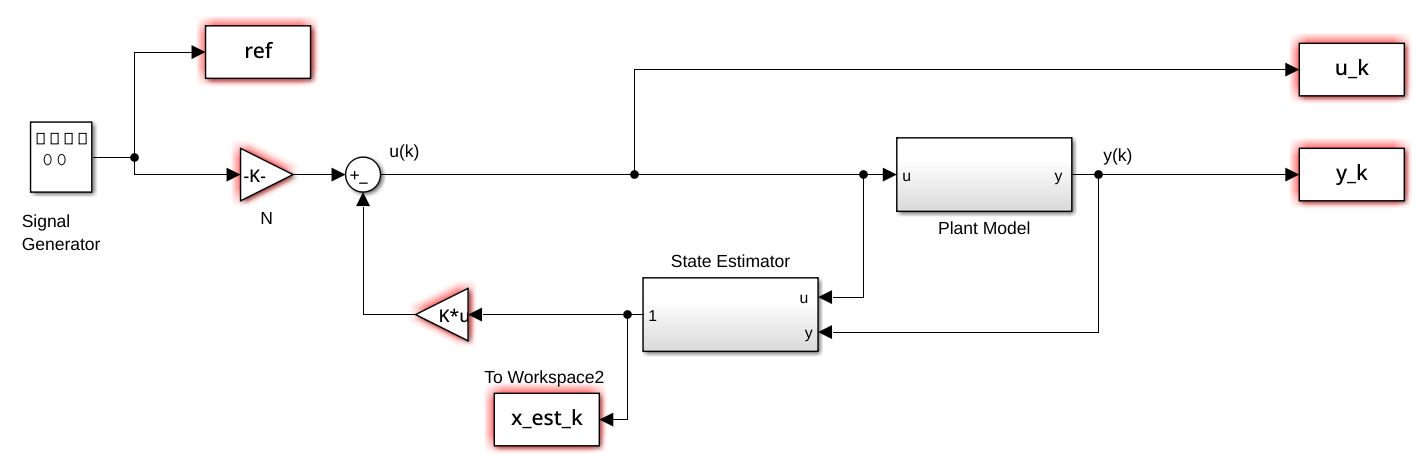
\includegraphics[width=0.9\textwidth]{Figs/Simulink Models/Controller_without_integrator.png}
        \caption{Controller without integrator}
        \label{fig:controller_without_integrator}
    \end{subfigure}
    \caption{Simulink models utilized for system control without integral action}
    \label{fig:simulink_models_no_integrator}
\end{figure}


\begin{figure}[H]
    \centering
    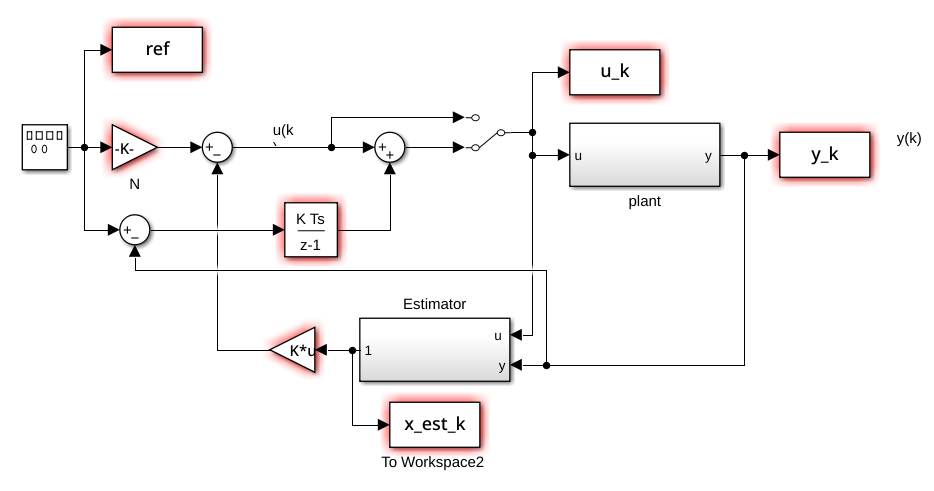
\includegraphics[width=0.7\textwidth]{Figs/Simulink Models/controller_with_integrator.png}
    \caption{Controller with integrator}
    \label{fig:controler_with_integrator}
\end{figure}
